\documentclass[11pt,review]{elsarticle}
\makeatletter
\def\ps@pprintTitle{%
 \let\@oddhead\@empty
 \let\@evenhead\@empty
 \def\@oddfoot{\centerline{\thepage}}%
 \let\@evenfoot\@oddfoot}
\makeatother

\usepackage[tmargin=1.25in,bmargin=1in,lmargin=1.25in,rmargin=1.25in]{geometry}

\usepackage[caption=false]{subfig}
\usepackage{booktabs}
\usepackage{threeparttable}

\usepackage{lineno,hyperref}
\modulolinenumbers[5]
\bibliographystyle{elsarticle-num}

\usepackage{amsmath,amssymb}
\usepackage{graphicx}
\graphicspath{{./figures/}}

\begin{document}

\begin{frontmatter}

\title{Title}
\author{Author 1}
\ead{email-1}
\address[ShortName]{Name of institution}
\author{Author 2}
\ead{email-2}
\address[ShortName]{Name of institution}

%\date{\today}

\begin{abstract}
Add abstract here
\end{abstract}

\begin{keyword}
Keyword 1 \sep keyword 2 \sep keyword 3 \sep keyword 4 \sep keyword 5
\end{keyword}

\end{frontmatter}

%\linenumbers

\section{Introduction}
Broad introduction

What is the paper about?

Previous work. Cite an article like this \cite{KO16}.

Highlights of the current approach

Outline of contents

\section{Methods} \label{sec:methods}

What are the mathematical / computational / experimental methods used in this work? Provide sufficient details in appropriate subsections

\subsection{Equations}

Inline and display equations are entered like this: consider the function $f:\mathbb{R} \to \mathbb{R}$ defined as

\begin{equation} \label{eq:fn_defn}
f(x) = \sin x.
\end{equation}

Multiple equations are entered like this:

\begin{equation} \label{eq:mult_eqns}
\begin{split}
(a + b)^3 &= (a + b)^2(a + b)\\
 &= (a^2 + 2ab + b^2)(a + b)\\
 &= a^3 + 3a^2 + 3ab^2 + b^3.
\end{split}
\end{equation}

Notice how equations are part of sentences. In particular, use appropriate punctuations like commas and periods, just as in a regular sentence.

\section{Results} \label{sec:results}

Systematically list out results in increasing order of complexity.

\subsection{Figures}

Figures are added like this: the function defined in Eq.~\eqref{eq:fn_defn} is plotted in Figure~\ref{fig:sine}.

\begin{figure}[h!]
\centering
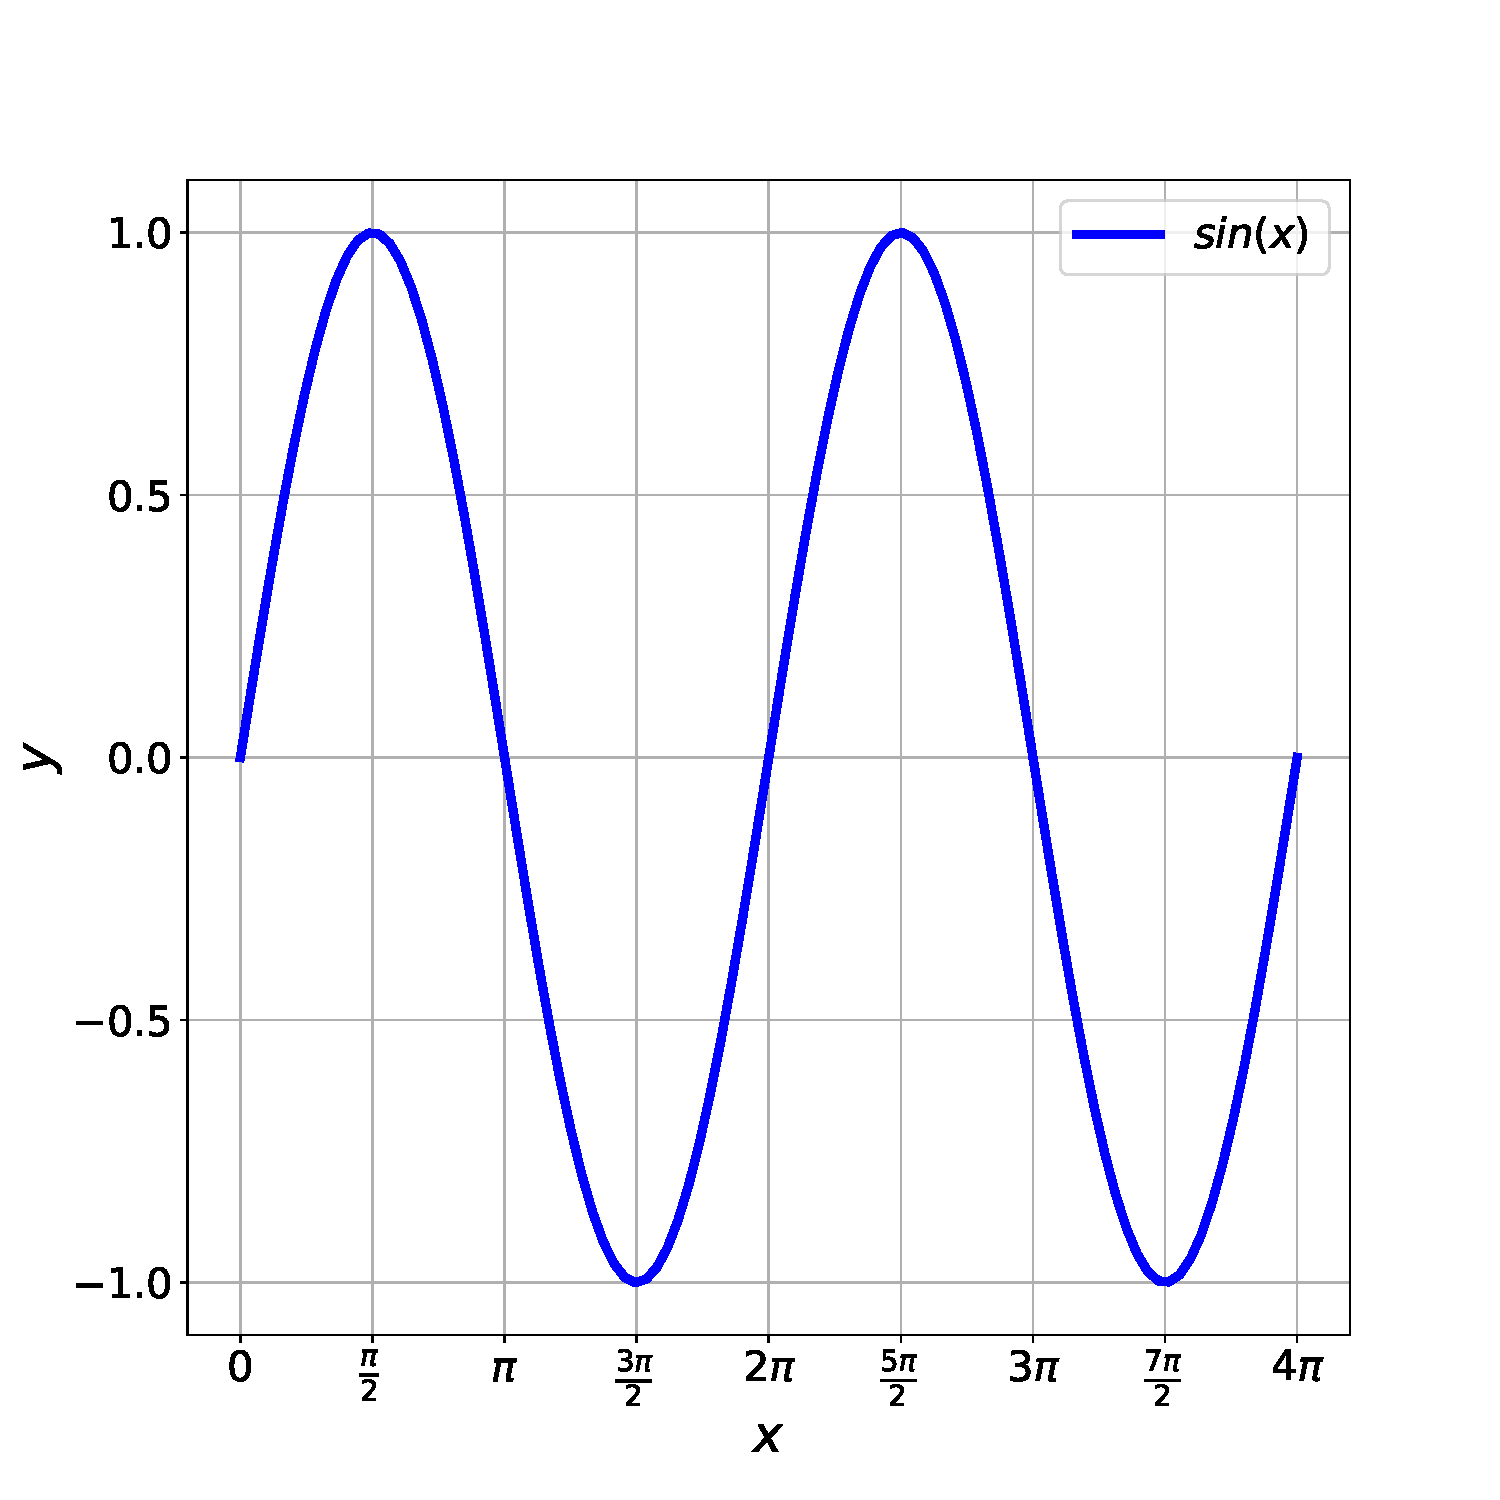
\includegraphics[width=0.5\textwidth]{Figures/sine.pdf}
\caption{Plot of the sine function over the interval $[0,4\pi]$.}
\label{fig:sine}
\end{figure}

Notice how the lines in Figure~\ref{fig:sine} are thick, and how the various fonts are bigger. This is necessary to make the figure readable.

\subsection{Tables}

Use the \texttt{threeparttable} package to create tables as shown in Table~\ref{tab:sine}.

\begin{table}
\centering
\begin{threeparttable}[b]
\begin{tabular}{cccc}
\toprule
$x$ & $\sin x$ & $\cos x$ & $\tan x$\\
\midrule
$0$ & $0$ & $1$ & $0$\\
$\frac{\pi}{6}$ & $\frac{1}{2}$ & $\frac{\sqrt{3}}{2}$ & $\frac{1}{\sqrt{3}}$\\
$\frac{\pi}{4}$ & $\frac{1}{\sqrt{2}}$ & $\frac{1}{\sqrt{2}}$ & $1$\\
$\frac{\pi}{3}$ & $\frac{\sqrt{3}}{2}$ & $\frac{1}{2}$ & $\sqrt{3}$\\
$\frac{\pi}{2}$ & $1$ & $0$ & $\infty$\\
\bottomrule
\end{tabular}
\end{threeparttable}
\caption{Some values of trigonometric functions in the interval $[0,\pi]$.}
\label{tab:sine}
\end{table}

\section{Discussion} \label{sec:discussion}
What do the results tell us? 

What implications do they have on this and related topics?

...

\section{Conclusion} \label{sec:conclusion}
Summarize and conclude the work

\section*{Acknowledgement}
Acknowledge funding sources and thank people who helped in the process of preparing the manuscript.

\section*{Declaration of Interest}
Declare competing interests if any.

\section*{References}

% The name of the bibligraphy file is bibfile.bib
\bibliography{bibfile}

\appendix

\section{Supplementary information} \label{app:si}

Add any supplementary information in one or more appendices. 

\end{document}